\begin{figure*}
\centering
\begin{tabular}{ccccc|c}
\hspace{-0.2cm}\includegraphics[width=0.2\textwidth]{../figures/additive_multi_d/additive_kernel_sum_p2.pdf} & \hspace{-0.4cm} + \hspace{-0.4cm} & 
\includegraphics[width=0.2\textwidth]{../figures/additive_multi_d/additive_kernel_sum_p1.pdf} & \hspace{-0.4cm} = \hspace{-0.4cm} & 
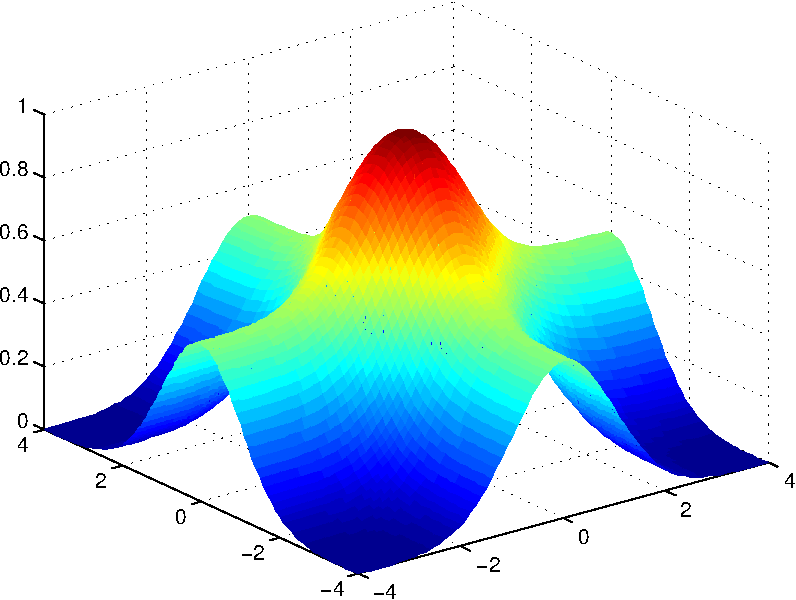
\includegraphics[width=0.2\textwidth]{../figures/additive_multi_d/additive_kernel.pdf} &
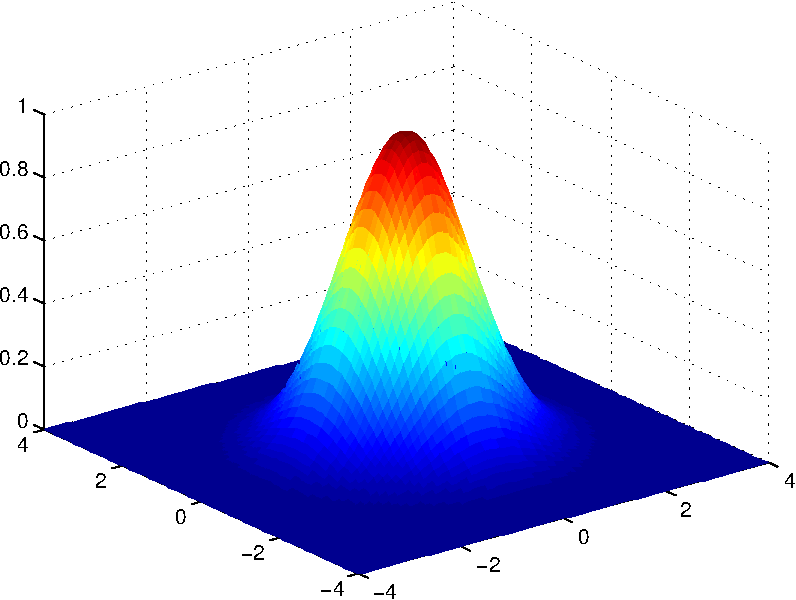
\includegraphics[width=0.2\textwidth]{../figures/additive_multi_d/sqexp_kernel.pdf} \\
$k_1(x_1, x_1')$ & & $k_2(x_2, x_2')$ & & $k_1(x_1,x_1') + k_2(x_2,x_2')$ &$k_1(x_1,x_1')k_2(x_2,x_2')$ \\
1D kernel & & 1D kernel & & sum of kernels & product of kernels \\ 
%& & & & & \\
%(Second Order) & & & & & Additive Kernel \\
$\downarrow$ & & $\downarrow$ & & $\downarrow$ & $\downarrow$ \\
\hspace{-0.2cm}\includegraphics[width=0.2\textwidth]{../figures/additive_multi_d/additive_kernel_draw_sum_p1.pdf}& \hspace{-0.4cm} + \hspace{-0.4cm}& 
\includegraphics[width=0.2\textwidth]{../figures/additive_multi_d/additive_kernel_draw_sum_p2.pdf}& \hspace{-0.4cm} = \hspace{-0.4cm}&
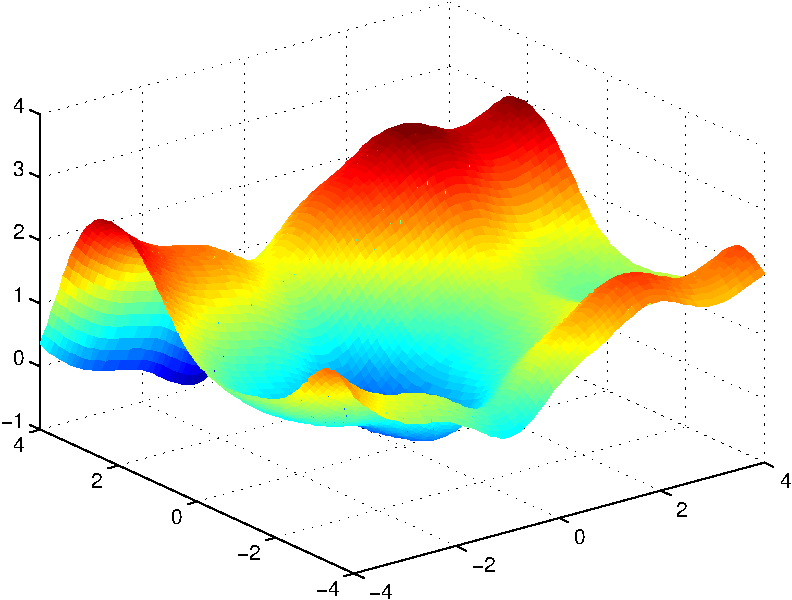
\includegraphics[width=0.2\textwidth]{../figures/additive_multi_d/additive_kernel_draw_sum.pdf} &
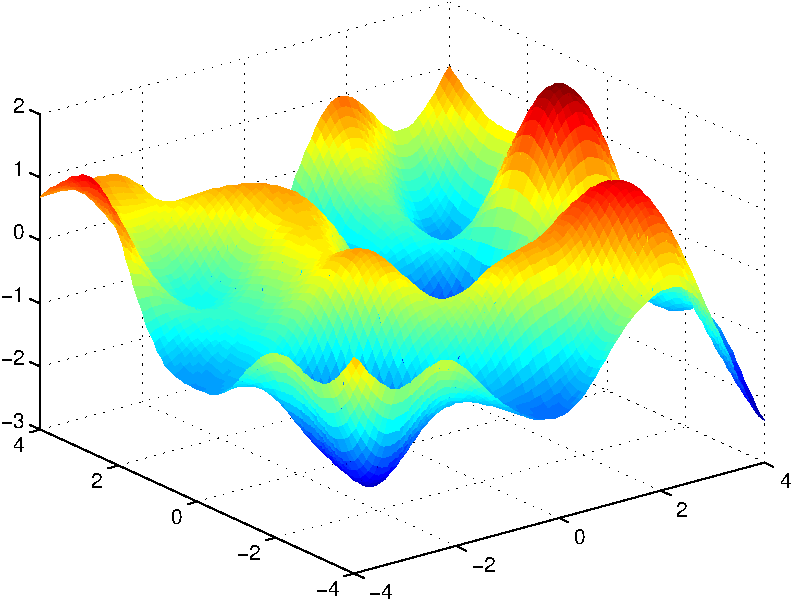
\includegraphics[width=0.2\textwidth]{../figures/additive_multi_d/sqexp_draw.pdf} \\
$f_1(x_1)$ & & $f_2(x_2)$ & & $f_1(x_1) + f_2(x_2)$ & $f(x_1, x_2)$ \\
draw from & & draw from & & draw from & draw from\\
1D GP prior & & 1D GP prior & & additive GP prior & product GP prior\\
%Draw from product kernel GP prior & Draw from additive kernel GP prior\\
\end{tabular}
\caption{A two-dimensional additive kernel, and a two-dimesnional product kernel.  Left: a draw from an additive kernel corresponds to a sum of draws from one-dimensional kernels.  Right: functions drawn from a product kernel prior have less long-range dependency.
%In this example, both kernels are composed of one dimensional squared-exponential kernels, but this need not be the case in general.
}
\label{fig:multi_d_additivity}
\end{figure*}
